%texexptitled======================================================================
% lab1-gcd
%-----------------------------------------------------------------------
%

\documentclass[11pt]{article}

% Package includes

\usepackage{graphicx}
\usepackage{color}
\usepackage{comment}
\usepackage{multirow}
\usepackage{askmaps}
\usepackage{amssymb}
\usepackage{amsmath}
\usepackage{tikz}
\usepackage{circuitikzgit}
\usetikzlibrary{arrows, positioning, shapes.geometric, circuits.logic.US}
\tikzstyle{line}=[draw]
\tikzstyle{arrow}=[draw, -latex]

% Wrap long URLs with hyphens
\PassOptionsToPackage{hyphens}{url}\usepackage{hyperref}
\usepackage{pdftexcmds}
\usepackage{upquote}
\usepackage{textcomp}
\usepackage{minted}
\usepackage[listings]{tcolorbox}
\usepackage{enumerate}
\usepackage{enumitem}
\usepackage{mathtools}
\DeclarePairedDelimiter{\ceil}{\Big\lceil}{\Big\rceil}

\tcbset{
texexp/.style={colframe=black, colback=lightgray!15,
         coltitle=white,
         fonttitle=\small\sffamily\bfseries, fontupper=\small, fontlower=\small},
     example/.style 2 args={texexp,
title={Question \thetcbcounter: #1},label={#2}},
}

\newtcolorbox{texexp}[1]{texexp}
\newtcolorbox[auto counter]{texexptitled}[3][]{%
example={#2}{#3},#1}

\setlength{\topmargin}{-0.5in}
\setlength{\textheight}{9in}
\setlength{\oddsidemargin}{0in}
\setlength{\evensidemargin}{0in}
\setlength{\textwidth}{6.5in}

% Useful macros

\newcommand{\note}[1]{{\bf [ NOTE: #1 ]}}
\newcommand{\fixme}[1]{{\bf [ FIXME: #1 ]}}
\newcommand{\wunits}[2]{\mbox{#1\,#2}}
\newcommand{\um}{\mbox{$\mu$m}}
\newcommand{\xum}[1]{\wunits{#1}{\um}}
\newcommand{\by}[2]{\mbox{#1$\times$#2}}
\newcommand{\byby}[3]{\mbox{#1$\times$#2$\times$#3}}


\newenvironment{tightlist}
{\begin{itemize}
 \setlength{\parsep}{0pt}
 \setlength{\itemsep}{-2pt}}
{\end{itemize}}

\newenvironment{titledtightlist}[1]
{\noindent
 ~~\textbf{#1}
 \begin{itemize}
 \setlength{\parsep}{0pt}
 \setlength{\itemsep}{-2pt}}
{\end{itemize}}

% Change spacing before and after section headers

\makeatletter
\renewcommand{\section}
{\@startsection {section}{1}{0pt}
 {-2ex}
 {1ex}
 {\bfseries\Large}}
\makeatother

\makeatletter
\renewcommand{\subsection}
{\@startsection {subsection}{1}{0pt}
 {-1ex}
 {0.5ex}
 {\bfseries\normalsize}}
\makeatother

% Reduce likelihood of a single line at the top/bottom of page

\clubpenalty=2000
\widowpenalty=2000

% Other commands and parameters

\pagestyle{myheadings}
\setlength{\parindent}{0in}
\setlength{\parskip}{10pt}

% Commands for register format figures.

\newcommand{\instbit}[1]{\mbox{\scriptsize #1}}
\newcommand{\instbitrange}[2]{\instbit{#1} \hfill \instbit{#2}}

\newif\ifsolution

\if\issolution1
\newenvironment{solution}
    {\color{red}}
    {\color{black}}
\solutiontrue
\else
\excludecomment{solution}
\solutionfalse
\fi


\graphicspath{{./figs/}}


%-----------------------------------------------------------------------
% Document
%-----------------------------------------------------------------------

\begin{document}
\def\PYZsq{\textquotesingle}


\newcommand{\headertext}{EE142 Problem Set 8}
\renewcommand{\thesubsection}{\thesection.\alph{subsection}}

\title{\vspace{-0.4in}\Large \bf \headertext \vspace{-0.1in}}
\author{Vighnesh Iyer}

\date{\today}
\maketitle

\markboth{\headertext}{\headertext}
\thispagestyle{empty}

\section{System Analysis}
{\color{blue}A wireless receiver front-end is shown below:}
\begin{figure}[H]
    \centering 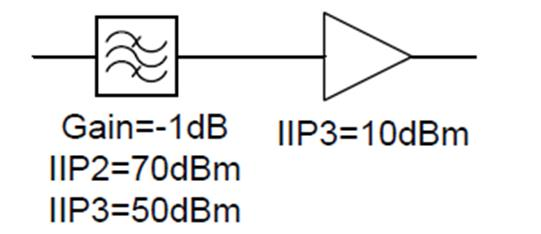
\includegraphics[width=\textwidth-8cm]{problem1_schematic1.jpg}
\end{figure}

{\color{blue}We would like to receive the channel at 1800MHz, while we have additional chanels at 900MHz, 1805MHz, and 1810MHz.}
\begin{figure}[H]
    \centering 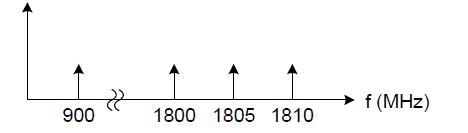
\includegraphics[width=\textwidth-5cm]{problem1_schematic2.jpg}
\end{figure}

{\color{blue}The minimum detectable signal at 1800MHz is -100dBm.
The required signal to distortion ratio at the front-end output is 9dB.}

\begin{enumerate}[label=(\alph*)]
    \item {\color{blue}If the signal power at the 1810MHz channel is -33dBm, what is the maximum allowed power at the 1805MHz channel?}

    We can find the cascaded IIP3 of the front-end:
    \begin{align*}
        \frac{1}{IIP3^2} = \frac{1}{IIP3_A^2} + \frac{a_1^2}{IIP3_B^2}
    \end{align*}

    where the $IIP3$ terms in the above formula are voltages or currents.

    Here are some useful equations to convert power to voltage, and convert power gain to voltage gain:
    \begin{align*}
        \text{Power Gain in dB} &= 10 \log_{10}(\text{Power Gain in Linear Units}) \\
        \text{Power Gain in Linear Units} &= 10^{\text{Power Gain in dB} / 10} \\
        \text{Voltage Gain} &= \sqrt{\text{Power Gain in Linear Units}} \text{ assuming same } R_{in}, R_{out} \\
        \text{Power in dBm} &= 10 \log_{10}(\frac{\text{Power in Watts}}{10^{-3}}) \\
        \text{Voltage Induced} &= \sqrt{10^{-3} \cdot 10^{\text{Power in dBm}/10} \cdot 2R} \\
        \text{Power Delivered in dBm} &= 10 \cdot \log_{10}(\frac{V^2}{2R} / 10^{-3})
    \end{align*}

    We will assume operation in a $50\Omega$ environment.
    \begin{align*}
        IIP3_A &= 50 \text{ dBm} \rightarrow VIIP3_A = 100 \text{ V} \\
        IIP3_B &= 10 \text{ dBm} \rightarrow VIIP3_B = 1 \text{ V} \\
        a_1 &= 0.8912 \text{ V/V} \\
        VIIP_3 &= 1.1219 \text{ V} \\
        IIP_3 &= 11 \text{ dBm}
    \end{align*}

    As expected, the second stage's IIP3 dominates the cascaded IIP3.
    The power present at 1800MHz is caused by the intermodulation products of 1805MHz and 1810MHz:
    \begin{align*}
        V_{out,1800} = \frac{3 a_3}{4} A_{1805}^2 \cdot A_{1810}
    \end{align*}

    where $A_{x}$ is the voltage at $x$ MHz. We can find $a_3$ from IIP3:
    \begin{align*}
        IIP3 &= \sqrt{\frac{4}{3} \frac{|a_1|}{|a_3|}} \\
        a_3 &= 0.944 \\
        V_{out,1800} \leq V(-109 dBm) &\rightarrow P_{1805} \leq -26.5 \text{ dBm}
    \end{align*}

    \item {\color{blue}What is the required spec for the amplifier IIP2 if the signal power at the 900MHz channel can be as high as -30dBm?}
\end{enumerate}

\section{Distortion Analysis}
{\color{blue} In this problem you will do distortion analysis for a frequency-independent amplifier.}
\begin{figure}[H]
    \centering 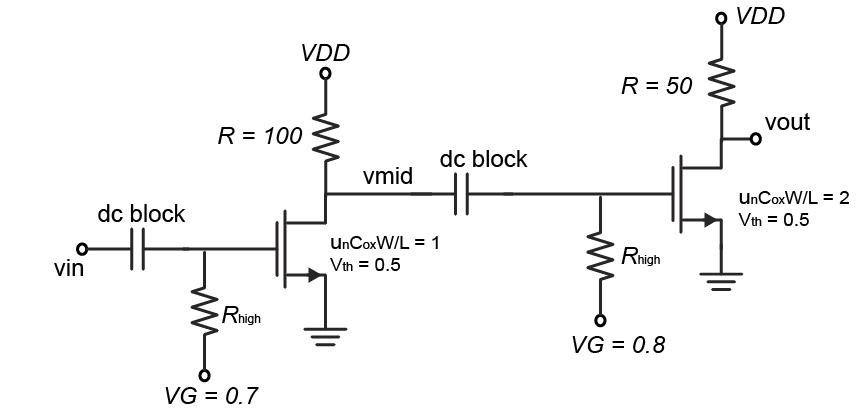
\includegraphics[width=\textwidth-5cm]{problem2_schematic.jpg}
\end{figure}

\begin{enumerate}[label=(\alph*)]
    \item {\color{blue} For the above amplifier, derive a power series to express the small-signal output voltage $v_{out}$ as a function of the small-signal input voltage $v_{in}$. Assume the transistors are long-channel devices.}

    We first derive the results for a single stage in general:
    \begin{align*}
        I_D &= \frac{1}{2} \mu_n C_{ox} \frac{W}{L} (V_{gs} - V_{th})^2 \\
        I_Q + i_{out} &= \frac{1}{2} \mu_n C_{ox} \frac{W}{L} (V_{GSQ} + v_{in} - V_{th})^2 \\
        I_Q + i_{out} &= 0.5 \mu_n C_{ox} W/L (V_{GSQ} - V_{th})^2 + \mu_n C_{ox} W/L (V_{GSQ} - V_{th})v_{in} + 0.5 \mu_n C_{ox} W/L \cdot v_{in}^2 \\
        i_{out} &= \mu_n C_{ox} W/L (V_{GSQ} - V_{th})v_{in} + 0.5 \mu_n C_{ox} W/L \cdot v_{in}^2 \\
        v_{out} &= i_{out} \cdot R
    \end{align*}

    Now consider the cascade:
    \begin{align*}
        v_{mid} &= (0.2 v_{in} + 0.5 v_{in}^2) \cdot 100 = 20 v_{in} + 50 v_{in}^2 \\
        v_{out} &= (0.6 v_{mid} + 1 v_{mid}^2) \cdot 50 \\
        v_{out} &= 600 v_{in} + 21500 v_{in}^2 + 100000 v_{in}^3 + 125000 v_{in}^4
    \end{align*}

    \item {\color{blue} Calculate IIP3 for the first stage ($v_{in}$ to $v_{mid}$), the second stage ($v_{mid}$ to $v_{out}$), and the overall cascade two-stage amplifier.}

    \begin{align*}
        VIIP3_A &= \sqrt{4/3 |a_1/a_3|} = \infty \\
        VIIP3_B &= \infty \\
        VIIP3_{cascade} &= 0.089 \text{ V} \rightarrow -11 \text{ dBm}
    \end{align*}

    \item {\color{blue} Find IIP2 for the first stage, the second stage, and the cascade two-stage amplifier.}

    \begin{align*}
        VIIP2_A &= \frac{a_1}{a_2} = 0.4 \text{ V} \rightarrow 2.04 \text{ dBm} \\
        VIIP2_B &= 0.6 \text{ V} \rightarrow 5.56 \text{ dBm} \\
        VIIP2_{cascade} &= 0.0279 \text{ V} \rightarrow -21 \text{ dBm} \\
    \end{align*}

    \item {\color{blue} Apply the cascade IIP3 and IIP2 formula introduced in the lecture. Explain if the results are different from that obtained via your analysis in part (b) and (c)}

    The cascade IIP2 formula yields the same result as derived explicitly, but the cascade IIP3 formula breaks down with infinite values and doesn't give the same answer as found in part (b).

    \item {\color{blue} Calculate HD2 and HD3 of this two-stage amplifier.}

    \begin{align*}
        HD_2 &= \frac{1}{2} \frac{a_2}{a_1} S_{in} = 18 \\
        HD_3 &= \frac{1}{4} \frac{a_3}{a_1} S_{in}^2 = 41.7
    \end{align*}

    \item {\color{blue} Use Harmonic Balance in ADS to simulate IIP2, IIP3, HD2, HD3 of this two-stage amplifier.}

    This is the setup in ADS:
    \begin{figure}[H]
        \centering 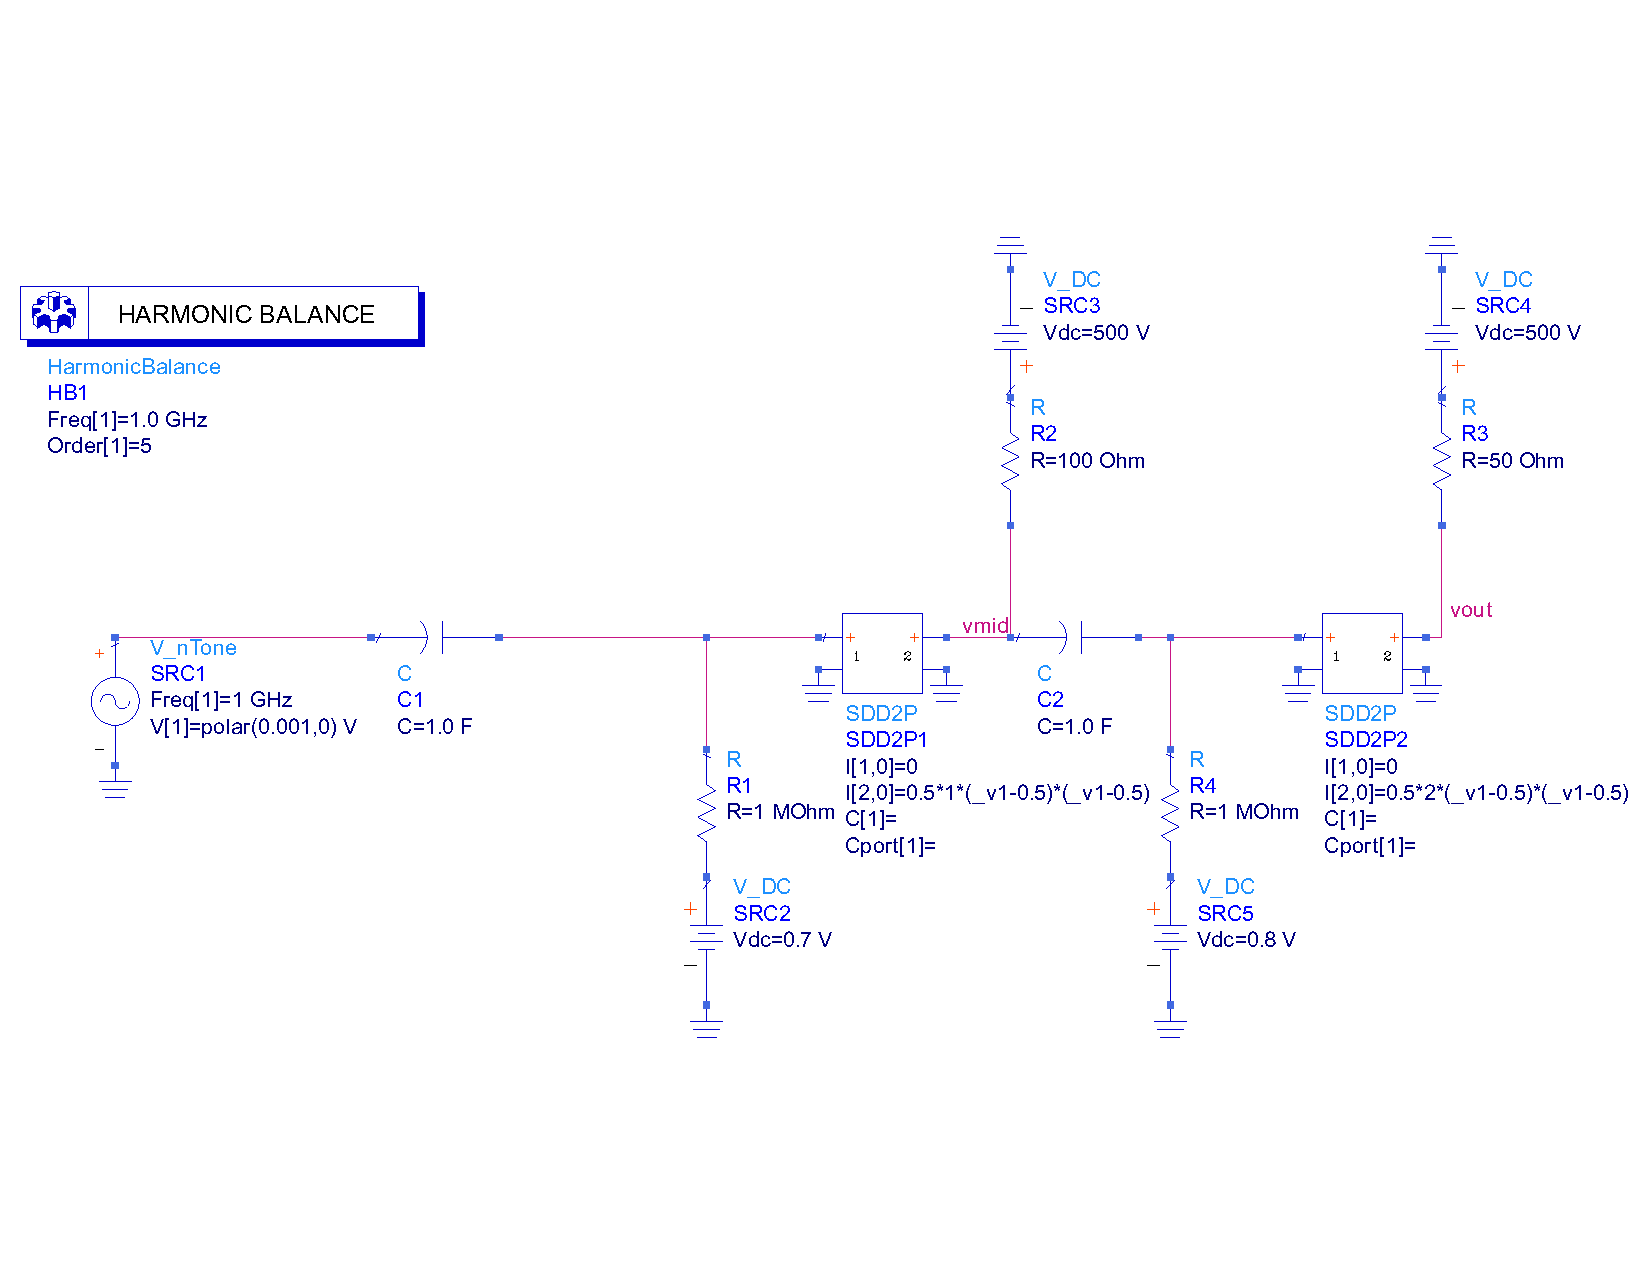
\includegraphics[width=\textwidth]{problem2_ads_schematic.pdf}
    \end{figure}

    We find from simulation that $a_1 = 600$, $a_2 = 18000$, and $a_3 = 100000$, which matches with the results derived by hand.
    From here, the IIP and HD numbers must also be the same.
\end{enumerate}

\section{Resonant Distortion Analysis}
{\color{blue} To achieve a higher output voltage swing, the two load resistors in the previous problem are replaced with 2 LC tanks, as illustrated.
Now perform distortion analysis for a tuned amplifier.
Keep in mind that in the passband of the amplifier (resonance), the memoryless assumption is valid.}
\begin{figure}[H]
    \centering 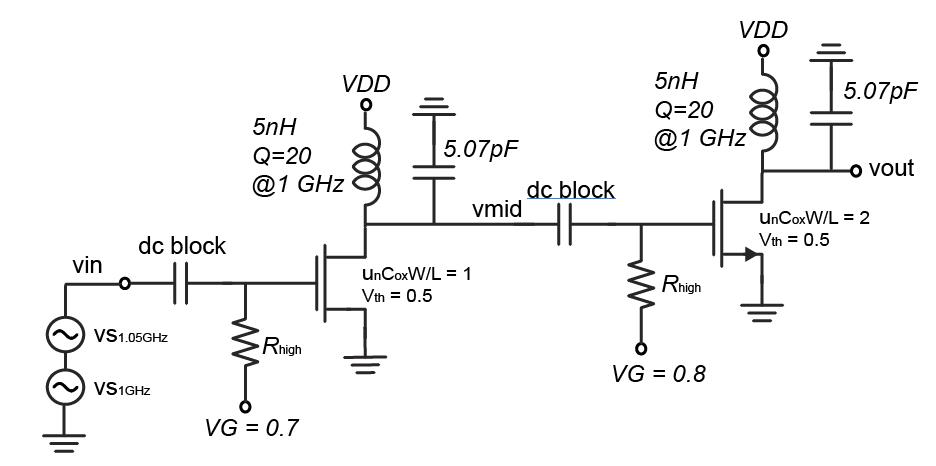
\includegraphics[width=\textwidth-5cm]{problem3_schematic.jpg}
\end{figure}
\begin{enumerate}[label=(\alph*)]
    \item {\color{blue} Under a two-tone excitation at 1.0 and 1.05 Ghz, with each having zero-to-peak voltage of 1mV, estimate the voltage components at 0.05, 0.95, 1, 1.05, 1.10, 2.0, and 3.0 Ghz at both $v_{mid}$ and $v_{out}$.}

    The characteristics of the transfer function are the same as in the previous problem, with the exception of the filtering going on, at $v_{mid}$ and the load resistance, which is replaced by the resistance of the inductor at resonance as defined by its component Q.

    The filtering that occurs at $v_{mid}$ only leaves behind frequencies near 1 GHz.
    We model what's going on as a memoryless non-linearity followed by a linear filter (which in hand calculation just kills everything away from 1GHz).
    The effective load resistance at resonance is determined by the $Q$ of the inductor.

    \begin{align*}
        Q_L = \frac{X_L}{R} = \frac{j \omega L}{R} = 20 \rightarrow R \rvert_{\omega = 1GHz} &= 1.571 \Omega \\
        \text{Series to Parallel Conv } \rightarrow R_p &= 630 \Omega
    \end{align*}

    Derive the full form of $v_{mid}$ for a 2-tone input on $v_{in}$ with voltage $A$:
    \begin{align*}
        v_{mid} = 2 A^{2} R a_{2} \cos{\left (\omega_1 t \right )} \cos{\left (\omega_2 t \right )} + \frac{R a_{2}}{2} A^{2} \cos{\left (2 \omega_1 t \right )} + \frac{R a_{2}}{2} A^{2} \cos{\left (2 \omega_2 t \right )} \\ + A^{2} R a_{2} + A R a_{1} \cos{\left (\omega_1 t \right )} + A R a_{1} \cos{\left (\omega_2 t \right )}
    \end{align*}

    We can immediately spot terms to throw away. The only terms to keep involve only $\omega_1$ and $\omega_2$. Everything else
        lies way beyond the 'passband' of the LC tank.
    \begin{align*}
        v_{mid,filtered} = A R a_{1} (\cos{\left (\omega_1 t \right )} + \cos{\left (\omega_2 t \right )}) \\
        v_{out} = A R^{2} a_{1} b_{1} \cos{\left (\omega_1 t \right )} + A R^{2} a_{1} b_{1} \cos{\left (\omega_2 t \right )}
    \end{align*}

    By the same token, we can throw away high/low frequency terms when deriving $v_{out}$. Voltage estimates:

    \begin{center}
    \begin{tabular}{| l | l |} \hline
        Freq & Voltage \\ \hline
        0.05 & 0 \\ \hline
        0.95 & 0 \\ \hline
        1 & 47.628 \\ \hline
        1.05 & 47.628 \\ \hline
        1.10 & 0 \\ \hline
        2.0 & 0 \\ \hline
        3.0 & 0 \\ \hline
    \end{tabular}
    \end{center}

    \item {\color{blue} Redo part (a) with $vs_{1.0GHz}$ reduced from 1 mV to 0.1 mV.}
    \begin{center}
    \begin{tabular}{| l | l |} \hline
        Freq & Voltage \\ \hline
        0.05 & 0 \\ \hline
        0.95 & 0 \\ \hline
        1 & 4.7628 \\ \hline
        1.05 & 47.628 \\ \hline
        1.10 & 0 \\ \hline
        2.0 & 0 \\ \hline
        3.0 & 0 \\ \hline
    \end{tabular}
    \end{center}
\end{enumerate}

\end{document}
